\documentclass[usenames,svgnames,14pt]{beamer}
\usepackage[english]{babel}
\usepackage{
  fontspec,
  fontawesome,
  xcolor,
  mathabx,
  listings,
  lstautogobble,
  listofitems,
  TeXnicalities,
  media9,
  array
}

\setsansfont{Yanone Kaffeesatz}[
    UprightFont     = *-Regular ,
    BoldFont        = *-Bold ,
    BoldItalicFont  = *-Bold ,
    BoldSlantedFont = *-Bold ,
    ItalicFont      = *-Light ,
    SlantedFont     = *-Light ,
    SmallCapsFont   = *-Thin
]
\graphicspath{{../Figures/}}
\usetheme[style=green]{Z02}

\usetikzlibrary{
    positioning,
    shapes,
    bbox
}
%Colors for listings
\colorlet{background-color}{gray!20}
\colorlet{basic-color}{black}
\colorlet{keywords-color}{Goldenrod}
\colorlet{comment-color}{red!95!black}
\colorlet{strings-color}{ForestGreen}
\colorlet{builtins-color}{MediumBlue!90!black}
\colorlet{functions-color}{NavyBlue}
\colorlet{variables-color}{DarkOrange}
\colorlet{environment-color}{Gray}
\colorlet{external-color}{SteelBlue}

% https://tex.stackexchange.com/a/34000
\makeatletter
\lst@Key{countblanklines}{true}[t]%
    {\lstKV@SetIf{#1}\lst@ifcountblanklines}

\lst@AddToHook{OnEmptyLine}{%
    \lst@ifnumberblanklines\else%
       \lst@ifcountblanklines\else%
         \advance\c@lstnumber-\@ne\relax%
       \fi%
    \fi}
\makeatother

%listings set
\lstdefinestyle{MyBash}{
backgroundcolor=\color{background-color}, % choose the background color; you must add \usepackage{color} or \usepackage{xcolor}
breakatwhitespace=false,            % sets if automatic breaks should only happen at whitespace
breaklines=true,                    % sets automatic line breaking
captionpos=b,                       % sets the caption-position to bottom
deletekeywords={...},               % if you want to delete keywords from the given language
escapeinside={@|}{|@},              % if you want to add LaTeX within your code
extendedchars=true,                 % lets you use non-ASCII characters; for 8-bits encodings only,
                                    % does not work with UTF-8
frame=single,                       % adds a frame around the code
framerule=0pt,                      % Width of the frame rule
framesep=3pt,                       % separation around text
linewidth=\textwidth,               % defines the base line width for listings
xleftmargin=6mm,                    % Margin left
xrightmargin=6mm,                   % Margin right
numbers=left,                       % where to put the line-numbers; possible values are (none, left, right)
numberblanklines=false,             % suppress numbers on empty lines
countblanklines=false,              % NOT standard! Avoid counting empty lines: https://tex.stackexchange.com/a/34000
numbersep=8pt,                      % how far the line-numbers are from the code
numberstyle=\tiny\color{black},     % the style that is used for the line-numbers
rulecolor=\color{black},            % if not set, the frame-color may be changed on line-breaks within not-black text
                                    % (e.g. comments (green here))
showspaces=false,                   % show spaces everywhere adding particular underscores; it overrides 'showstringspaces'
showstringspaces=false,             % underline spaces within strings only
showtabs=false,                     % show tabs within strings adding particular underscores
stepnumber=1,                       % the step between two line-numbers. If it's 1, each line will be numbered
tabsize=2,                          % sets default tabsize to 2 spaces
title=\lstname,                     % show the filename of files included with \lstinputlisting; also try caption instead of title
%
%Base style for this presentation 
keepspaces=true,                    % keeps spaces in text, useful for keeping indentation of code
                                    % (possibly needs columns=flexible)
language=bash,
basicstyle=\ttfamily\scriptsize\color{basic-color},
keywordstyle=\color{keywords-color},
stringstyle=\color{strings-color},
commentstyle=\color{comment-color},
morestring=[b][\color{strings-color}]{"},
morestring=[d][\color{strings-color}]{'},
moredelim=[is][\color{basic-color}]{|+}{+|}, % I will use this for terminal output
literate={`}{\textasciigrave}1, % https://tex.stackexchange.com/a/466224/128737
literate={~}{{\textasciitilde}}1,
% literate=% literate={<replace>}{<replacement text>}{<width>}
%   {\#define}{{{\color{CarnationPink}\#define}}}{6}
%   {\#include}{{{\color{CarnationPink}\#include}}}{7},
alsoletter=0123456789![]/\{\}.:+, % This to mark the symbols in keyword/emph[5] to be highlighted (otherkeywords does not work i.e. it highlights also in comments!) -> manual at page 45
morekeywords={if, then, else, elif, fi, case, esac, for, select, while, until, do, done, in, function, time, [[, ]], \{, \}, !, coproc}, %https://askubuntu.com/a/513712
emph=[1]{},
emphstyle=[1]{\color{functions-color}}, %Functions
emph=[2]{},
emphstyle=[2]{\color{variables-color}}, %Variables
emph=[4]{PATH, SHELL, IFS, BASH_ALIASES, BASH_REMATCH, PS3, REPLY, HOME, LANGUAGE, EDITOR, PIPESTATUS, PWD, FUNCNEST,
         DIRSTACK, PWD, OLDPWD, SHELLOPTS, BASHOPTS, TIMEFORMAT, COMP_CWORD, COMP_LINE, COMP_POINT, COMP_TYPE, COMP_KEY,
         COMP_WORDBREAKS, COMP_WORDS, COMPREPLY, INPUTRC},
emphstyle=[4]{\color{environment-color}}, %Environment variables
emph=[5]{alias, bg, bind, break, builtin, cd, command, compgen, complete, continue, declare, dirs, disown, echo, enable, eval,
         exec, exit, export, false, fc, fg, getopts, hash, help, history, jobs, kill, let, local, logout, popd, printf, pushd, pwd,
         read, readonly, return, set, shift, shopt, source, suspend, test, times, trap, true, type, typeset, ulimit, umask,
         % case, if, until, while  % <--- these built-in are keywords and I leave them highlighted as such
         unalias, unset, wait, :, ., [, ]},
emphstyle=[5]{\color{builtins-color}}, %Shell built-in
emph=[6]{man, apropos, ls, rm, g++, chmod, cp, awk, sed, cut, perl, args, date, grep, sleep, tput, seq, cat, wc, sort, uniq, tail,
         head, sdiff, tar, mktemp, mkdir, ps, emacs, systemd, timeout, parallel, xargs, gnuplot, pdflatex, vi, ping, bash,
         egrep, shuf, stat, find, fgrep, bc, tr, paste, expr, diff, touch},
emphstyle=[6]{\color{external-color}}, %(External) commands
emph=[7]{},
emphstyle=[7]{\color{variables-color}}, %Class for local variables (usually with bad names)
emph=[8]{},
emphstyle=[8]{\color{builtins-color}}, %Class for local commands (usually with bad names)
%
%Additional customizations
belowskip=-7mm,
aboveskip=3pt,
autogobble=true, % lstautogobble needed!
}

\lstnewenvironment{Bash}[1][] %I will rarely use this because putting a $ in it as prompt breaks down TeXclipse highlight syntax!
    {\lstset{style=MyBash, #1}}
    {}

\def\bash{\lstinline[style=MyBash, basicstyle=\ttfamily\color{black}]}

%\includeonlyframes{current}

%===============================================================%
\title{Let's Git together}
\date{6 July 2023}
\author{Alessandro Sciarra}
\institute{CRC-TR\,211~--~Software Development Center}
\titlegraphic{
\includegraphics[width=16mm]{LogoCRC}}
\titlepagelogo{
\includegraphics[width=25mm]{LogoGoethe}}
%===============================================================%

\AtBeginSection[] % <- Empty optional argument, do nothing for \section*
{
    \begin{frame}[plain, noframenumbering]{}
         \sectionpage
    \end{frame}
}

\tikzset{
    space/.style={%
        thick, draw=#1, fill=#1!10, text=#1, rounded corners=1mm, font=\small, text width=14mm, align=center, minimum height=12mm
    },
    commit/.style={circle, draw, very thick, fill=#1, minimum size=5mm},
    branch/.style={rounded corners=1mm, fill=#1, draw, very thick, font=\small},
    pin/.style={to, thick, shorter={1pt}{1pt}}
}
\PrepareURLsymbol[PB]
\newcommand{\ttc}[2]{\texttt{\textcolor{#1}{#2}}}%
\setlength{\leftmarginii}{0.5cm}
\newcommand{\then}{\raisebox{2pt}{$\;\drsh\;$}}


% Taken from https://tex.stackexchange.com/a/51458/128737
\makeatletter
\patchcmd{\beamer@sectionintoc}{\vskip1.5em}{\vskip0.5em}{}{}
\makeatother

\begin{document}

%===============================================================%
\begin{frame}[plain,noframenumbering]
    \titlepage
    \begin{tikzpicture}[remember picture, overlay]
        \node[anchor=south, inner ysep=4pt] at ($(current page.south)!0.58!(current page.south east)+(0mm,1mm)$)
        {
\includegraphics[width=13mm]{LogoPUNCH}};
        \node[anchor=south, inner ysep=0pt] (license) at ($(current page.south)+(0mm,4mm)$)
        {
\includegraphics[width=10mm]{CC-BY}};
        \node[anchor=south, font=\small, text=BGLIGHT]
        (Axel) at (license.north)
        {\href{https://github.com/AxelKrypton}{\faGithub\,AxelKrypton}};
    \end{tikzpicture}
\end{frame}
%~~~~~~~~~~~~~~~~~~~~~~~~~~~~~~~~~~~~~~~~~~~~%
\begin{frame}{Outline of the talk}
    \tableofcontents[subsectionstyle=hide]
\end{frame}
%===============================================================%



%===============================================================%
\section{A short recap from last time}
%~~~~~~~~~~~~~~~~~~~~~~~~~~~~~~~~~~~~~~~~~~~~%
\begin{frame}{By now, this is how your workflow looks like}
    \begin{center}
        \begin{tikzpicture}[node distance=3mm, bezier bounding box] % \usetikzlibrary{bbox}
            \coordinate (N0) at (0,0);
            \foreach \n/\c [count=\i from 0, count=\ip from 1] in {Work/PS, git status git diff/PP, git add/PB, git commit/PT}{
                \begin{scope}[scope on=<1->]
                    \node[space=\c, below = of N\i, xshift=25mm] (N\ip) {\n};
                    \ifnum\i>0%
                    \path[thick, to] (N\i.east) edge[out=0, in=90] (N\ip.north);
                    \fi
                \end{scope}
            }
            \path[visible on=<1->, thick, dotted, to] (N4.west) edge[out=180, in=180, looseness=1.6] (N2.west);
            \path[visible on=<1->, thick, to] (N4.south) edge[out=270, in=180, looseness=1.3] (N1.west);
        \end{tikzpicture}
    \end{center}
\end{frame}
%~~~~~~~~~~~~~~~~~~~~~~~~~~~~~~~~~~~~~~~~~~~~%
\newcommand{\GitCommand}[6][midway]{%
    \draw[#2] ($(N#3.south)!#5!(E#3)$) -- node[#1, fill=BGLIGHT, font=\ttfamily\scriptsize] {#6} ($(N#4.south)!#5!(E#4)$);
}
\begin{frame}{Our mental picture, so far}{On your local machine}
    \vspace{-0.1\textheight}
    \begin{center}
        \begin{tikzpicture}[node distance=25mm]
            \begin{scope}[scope on=<1->]
                \coordinate (N0) at (0,0);
                \foreach \n/\c [count=\i from 0, count=\ip from 1] in {Workspace/PS, Staging area/PP, Local repository/PB}{
                    \node[space=\c, right = of N\i] (N\ip) {\n};
                    \draw[very thin] (N\ip) -- coordinate[pos=1] (E\ip) ++(0,-5);
                }
            \end{scope}
            \begin{scope}[scope on=<1->]
                \node[text=PQ, font=\ttfamily\scriptsize] at ($(N1)!0.5!(N2)$) {git status};
                \node[text=PQ, font=\ttfamily\scriptsize] at ($(N3.north)+(0,0.3)$) {git log};
                \node[text=PQ, font=\ttfamily\scriptsize] at ($(N3.north)+(0,0.7)$) {git show};
                \GitCommand{fromto,PQ}{1}{2}{0.10}{git diff}
                \GitCommand{fromto,PQ}{2}{3}{0.25}{git diff --staged}
                \GitCommand{to}{1}{2}{0.65}{git add}
                \GitCommand{from}{1}{2}{0.80}{git restore --staged}
                \GitCommand{to}{2}{3}{0.95}{git commit}
                \path[to, PQ] ($($(N3.south)!0.45!(E3)$)!0.65!($(N2.south)!0.45!(E2)$)$) edge[out=180, in=0] ($(N2.south)!0.35!(E2)$);
                \GitCommand[pos=0.8]{fromto,PQ}{1}{3}{0.45}{git diff HEAD}
                \node[text=PT] at ($($(N1.south)!0.47!(E1)$)!0.8!($(N3.south)!0.51!(E3)$)$) {\Remark{only tracked files}};
            \end{scope}
        \end{tikzpicture}
        \par\medskip
        {\small Commands marked in \PQ{dark red} do not change anything in the repository!}
        \FrameRemark{Git introduced \texttt{git-restore} in v2.23 but this stayed buggy for a while. Use it from v2.27 on, otherwhise use \texttt{git-reset}.}
    \end{center}
\end{frame}
%~~~~~~~~~~~~~~~~~~~~~~~~~~~~~~~~~~~~~~~~~~~~%
\newsavebox{\lstclonebox}
\begin{frame}<1-3>[fragile,label=MentalPicture]
    \frametitle<1-3>{The complete correct abstract mental setup}
    \frametitle<4->{Cloning a remote repository}
    \begin{lrbox}{\lstclonebox}
        \begin{lstlisting}[style=MyBash]
            # Clone, i.e. download, a remote repository in present directory
            $ git clone |+<path-or-url-to-repository> [<optional-folder-name>]+|
        \end{lstlisting}
    \end{lrbox}
    \begin{tikzpicture}[node distance=5mm]
        \coordinate (N0) at (0,0);
        \foreach \n/\c [count=\i from 0, count=\ip from 1] in {Stashing area/PQ, Workspace/PS, Staging area/PP, Local repository/PB, Remote repository/PT}{
            \node[space=\c, right = of N\i] (N\ip) {\n};
            \draw[very thin] (N\ip) -- coordinate[pos=1] (E\ip) ++(0,-5);
        }
        \path coordinate (DNE) at ($(N4.north east)!0.5!(N5.north west)+(0,1)$)
              coordinate (DSE) at ($(DNE)-(0,7.1)$)
              coordinate (DNW) at ($(N1.north east)!0.5!(N2.north west)+(0,1)$)
              coordinate (DSW) at ($(DNW)-(0,7.1)$);
        \draw[thin, dashed] (DNE) -- (DSE);
        \draw ($(N1.north west)-(0.1,0)$) -- ++(0,0.2) -| ($(N4.north east)+(0.1,0)$);
        \node[font=\small, anchor=south, inner sep=0pt] at ($(N1.north)!0.5!(N4.north)+(0,0.4)$) {Local machine};
        \node[draw=red, very thick, rounded corners=1mm, fill=yellow, text width=0.9\textwidth, align=center, font=\bfseries\large, text=red, visible on=<3>]
            at ($(N3.south)!0.5!(E3)$) {It's all about having this picture clear in mind and understand how git commands affect it};
        \begin{onlyenv}<1>
            \fill[Gray, fill opacity=0.95] (DNW) rectangle ($(DSW)-(2.3,0)$) node[pos=0.5, rotate=90, text=BGLIGHT, font=\large\bfseries] {Next part of the course};
            \fill[Gray, fill opacity=0.95] (DNE) rectangle ($(DSE)+(2.3,0)$) node[pos=0.5, rotate=90, text=BGLIGHT, font=\large\bfseries] {Next part of the course};
        \end{onlyenv}
        \node[visible on=<1-3>] at ($(DSW)!0.5!(DSE)-(0,0.3)$) {\alt<1>{What we explored last time}{Now we'll complete the picture}};
        % Second slide
        \fill[Gray, fill opacity=0.98, visible on=<4>] ($(DNW)-(2.3,0)$) rectangle ($(DSE)-(0,0)$) node[pos=0.5, rotate=37, text=BGLIGHT, font=\large\bfseries] {Nothing existing before cloning the remote repository};
        \node[visible on=<5>] at ($(N3.south)!0.5!(E3)-(0.1,0)$) {\usebox{\lstclonebox}};
    \end{tikzpicture}
\end{frame}
%===============================================================%


%===============================================================%
\section{Using branches}
%~~~~~~~~~~~~~~~~~~~~~~~~~~~~~~~~~~~~~~~~~~~~%
\begin{frame}[label=current]{A key feature of Git}
    \begin{overlayarea}{\textwidth}{0.7\textheight}
        \begin{itemize}
            \item Branches store \textbf{different versions of your project}
            \item Technically just pointers to a commit\\[2\itemsep]
                  \begin{onlyenv}<1>
                      \vspace{2mm}
                      \begin{tikzpicture}
                          \draw[very thick] (0,0) -- (5.2,0) (5.2,-1.2) -- (7.6,-1.2);
                          \foreach \x [count=\i from 1] in {0,2,3.2,5.2}{
                              \node[commit=PS!50] (M\i) at (\x,0) {};
                          }
                          \foreach \x [count=\i from 1] in {5.2,6.4,7.6}{
                              \node[commit=PP!70] (B\i) at (\x,-1.2) {};
                          }
                          \node[commit=PT!80] (L) at (2,1.2) {};
                          % Branch labels
                          \node[above = of L, branch=PT!80] (BrA) {Feature A};
                          \node[above = of M4, branch=PS!50] (BrM) {Main};
                          \node[above = of B3, branch=PP!70] (BrB) {Feature B};
                          % Complete paths
                          \path[very thick] (0.7,0) edge[out=0, in=180] (L.west);
                          \path[very thick] (3.9,0) edge[out=0, in=180] (B1.west);
                          \draw[pin] (BrA.south) -- (L.north);
                          \draw[pin] (BrM.south) -- (M4.north);
                          \draw[pin] (BrB.south) -- (B3.north);
                      \end{tikzpicture}
                  \end{onlyenv}
            \item<2-> They enable parallel development
                  \begin{itemize}
                      \item Implement new features
                      \item Fix bugs
                      \item Try out something
                      \item {}[\ldots]
                  \end{itemize}
            \item<2-> The always existing \;\PB{\texttt{main}}\; branch:
                  \begin{itemize}
                      \item By default created at initialization
                      \item Development should be done on other branches
                      \item Till \textasciitilde2020 it was called \;\PB{\texttt{master}}
                  \end{itemize}
        \end{itemize}
    \end{overlayarea}
\end{frame}
%~~~~~~~~~~~~~~~~~~~~~~~~~~~~~~~~~~~~~~~~~~~~%
\begin{frame}[fragile]{Git branch}
    \begin{lstlisting}[style=MyBash]
        # List all existing local branches
        $ git branch
        * |-main-|
    \end{lstlisting}
    \begin{lstlisting}[style=MyBash]
        # Create a new branch
        $ git branch new-branch
        $ git branch
        * |-main-|
        |+  new-branch+|
    \end{lstlisting}
    \begin{lstlisting}[style=MyBash]
        # Delete a branch
        $ git branch -d new-branch
        |+Deleted branch new-branch (was a45b032).+|
        $ git branch
        * |-main-|
    \end{lstlisting}
    \begin{varblock}{alert}[\textwidth]{Git is safe}
        \small
        If a modifications would be lost, Git does not allow you to delete the branch using the \texttt{-d} option.
        Use the \texttt{-D} option, instead, to force the deletion.
    \end{varblock}
\end{frame}
%~~~~~~~~~~~~~~~~~~~~~~~~~~~~~~~~~~~~~~~~~~~~%
\begin{frame}[fragile]{Git switch}
    \begin{overlayarea}{\textwidth}{0.8\textheight}
        \begin{varblock}{}[0.7\textwidth]{}
            \PB{This will in general change your workspace!}
        \end{varblock}
        \begin{lstlisting}[style=MyBash]
            # Switching to another branch
            $ git branch
            |+*+| |-main-|
            |+  new-branch+|
            $ git switch new-branch
            |+Switched to branch 'new-branch'+|
            $ git branch
            |+  main+|
            |+*+| |-new-branch-|
        \end{lstlisting}
        \begin{varblock}{alert}[\textwidth]{Git is safe}<only@1>
            \small
            You may switch branches with uncommitted changes in the work-tree if and only if said switching does not require clobbering those changes.
        \end{varblock}
        \begin{onlyenv}<2>
            \begin{lstlisting}[style=MyBash]
                # Creating and switching to a new branch at once
                $ git switch -c another-branch
                |+Switched to a new branch 'another-branch'+|
                $ git branch
                |+*+| |-another-branch-|
                |+  main+|                    # Pay attention from which
                |+  new-branch+|              # branch you create a new one!
            \end{lstlisting}
        \end{onlyenv}
    \end{overlayarea}
    \FrameRemark{Before v2.23 of Git (August 2019), the command \;\texttt{git checkout}\; needed to be used to switch branch.}
\end{frame}
%~~~~~~~~~~~~~~~~~~~~~~~~~~~~~~~~~~~~~~~~~~~~%
\begin{frame}{Merging branches}
    \setlength{\leftmargini}{0.6cm}
    \begin{itemize}
        \item To merge means to unify the snapshots of two different branches
        \item This is automatically done by Git in a clever way
        \item When Git does not know how to merge the content of some file, it will create a conflict
        \item If conflicts occur, the merge will not automatically finish
        \item A merge can be aborted in case of conflicts with the \,\texttt{--abort}\, option
              \Remark{The content of the repository will be restored to the state before issuing the merge command}
        \item To fix conflicts, open and manually adjust files where Git failed
    \end{itemize}
    \medskip
    \begin{varblock}{alert}[0.65\textwidth]{}
        \alert{Git is safe, conflicts are not a bad thing!}
    \end{varblock}
\end{frame}
%~~~~~~~~~~~~~~~~~~~~~~~~~~~~~~~~~~~~~~~~~~~~%
\newcommand{\commits}[2]{%
    \draw[very thick] (#1) -- ($(#1)+(2.5,0)$) edge[out=0, in=180] ($(#1)+(3.5,1)$);
    \draw[very thick] ($(#1)+(3.5,1)$) -- ($(#1)+(5,1)$);
    \foreach \dx/\dy [count=\i from 1] in {0/0, 1/0, 2/0, 4/1, 5/1}{
        \ifnum\i=#2
            \def\col{PS!50}
        \else
            \def\col{white}
        \fi
        \node[commit=\col] (C\i) at ($(#1)+(\dx,\dy)$) {};
    }
}

\begin{frame}{Different types of merge}
    \vspace{3mm}
    \resizebox{\textwidth}{!}{
        \begin{tikzpicture}
            \path coordinate (FF1S) at (0,0)
                  coordinate (FF2S) at (0,-4.5)
                  coordinate (3W1S) at (7,0)
                  coordinate (3W2S) at (7,-4.5);
            % Fast-forward before
            \commits{FF1S}{3}
            \draw[pin] ($(C3.north)+(0,1)$) -- node[pos=0, anchor=south,  branch=PS!50] (M) {Main} ++(0,-1);
            \draw[pin] ($(C5.north)+(0,1)$) -- node[pos=0, anchor=south,  branch=PP!50] (F) {Feature} ++(0,-1);
            \node[font=\large] (BL) at ($(FF1S)!0.5!(FF1S |- F)-(2,0)$) {\rotatebox{90}{Before merge}};
            \node[font=\Large] (FFL) at ($(FF1S |- F)!0.5!(F)+(0,1.5)$) {Fast-forward merge};
            % Fast-forward after
            \commits{FF2S}{5}
            \draw[pin] ($(C5.south)-(0,1)$) -- node[pos=0, anchor=north,  branch=PS!50] (M) {Main} ++(0,1);
            \draw[pin] ($(C5.north)+(0,1)$) -- node[pos=0, anchor=south,  branch=PP!50] (F) {Feature} ++(0,-1);
            \node[font=\large] (AL) at ($(FF2S |- M)!0.5!(FF2S |- F)-(2,0)$) {\rotatebox{90}{After merge}};
            % 3-way before
            \commits{3W1S}{0}
            \draw[pin] ($(C5.north)+(0,1)$) -- node[pos=0, anchor=south,  branch=PP!50] (F) {Feature} ++(0,-1);
            \draw[very thick] ($(3W1S)+(2.5,0)$) -- ++(1.5,0);
            \node[commit=PS!50] (C6) at ($(3W1S)+(4,0)$) {};
            \draw[pin] ($(C6.east)+(1,0)$) -- node[pos=0, anchor=west,  branch=PS!50] (M) {Main} ++(-1,0);
            % 3-way after
            \commits{3W2S}{0}
            \draw[pin] ($(C5.north)+(0,1)$) -- node[pos=0, anchor=south,  branch=PP!50] (F) {Feature} ++(0,-1);
            \draw[very thick] ($(3W2S)+(2.5,0)$) -- ++(4.5,0);
            \draw[very thick] ($(3W2S)+(5.25,1)$) -- ($(3W2S)+(5.5,1)$) edge[out=0, in=180] ($(3W2S)+(6.5,0)$);
            \node[commit=white]      at ($(3W2S)+(4,0)$) {};
            \node[commit=PS!50] (C7) at ($(3W2S)+(7,0)$) {};
            \draw[pin] ($(C7.north)+(0,1)$) -- node[pos=0, anchor=south,  branch=PS!50] (M) {Main} ++(0,-1);
            \node[font=\Large] (3WL) at ({$(3W2S)!0.5!(C7)$} |- FFL) {Three-way merge};
            % Final lines
            \draw (6.25,4.5) -- (6.25,-6);
            \draw (-2.5,-1) -- ++(17,0);
        \end{tikzpicture}
    }
    \FrameRemark{The \alert{three}-way nomenclature comes from the fact that Git uses three commits to generate the merge commit: the two branch tips and their common ancestor.}
\end{frame}
%~~~~~~~~~~~~~~~~~~~~~~~~~~~~~~~~~~~~~~~~~~~~%
\begin{frame}[fragile]{Git merge: How does it work?}
    \vspace{-3mm}
    \setlength{\leftmargini}{5mm}
    \begin{enumerate}
        \item If possible, Git performs a fast-forward merge
        \item Otherwise a three-way merge is done and a new commit created
    \end{enumerate}
    \begin{varblock}{}[0.75\textwidth]{Be sure to be on the correct branch!}
        \begin{lstlisting}[style=MyBash, xrightmargin=11mm, xleftmargin=11mm, aboveskip=2mm]
            |+   +|git merge |+<source-branch>+|
        \end{lstlisting}
        It incorporates changes from the specified\\ branch into the present branch!
    \end{varblock}
    \vspace{3mm}
    \begin{lstlisting}[style=MyBash]
        # It is possible to force a three-way merge:
        $ git merge --no-ff |+<source-branch>+|
    \end{lstlisting}
\end{frame}
%~~~~~~~~~~~~~~~~~~~~~~~~~~~~~~~~~~~~~~~~~~~~%
\begin{frame}[fragile]{Merge conflicts: Fixing procedure}
    \begin{lstlisting}[style=MyBash, xleftmargin=-1mm, xrightmargin=-1mm]
        # A general example
        $ git merge <branch_name>
        |+Auto-merging <file>
        CONFLICT (content): Merge conflict in <file>
        Automatic merge failed; fix conflicts and then commit the result.+|
    \end{lstlisting}
    \vspace{3mm}
    \begin{enumerate}
        \small
        \item Run \,\texttt{git status}\, to see \alert{unmerged paths}
        \item Find problematic hunks in files that contain conflicts\\
              \then Look for delimiters in the files:
              {~\footnotesize\texttt{<<<<<<<},\; \texttt{=======},\; \texttt{>>>>>>>}}
        \item Remove delimiters and adjust content
        \item Check the project works (e.g. compile, run tests)
        \item \texttt{git add}\, the files with fixed conflicts
        \item Commit added files\\
              \then Git propose you an auto-generated commit message
    \end{enumerate}
\end{frame}
%~~~~~~~~~~~~~~~~~~~~~~~~~~~~~~~~~~~~~~~~~~~~%
\AlertFrame{Live example!}
%~~~~~~~~~~~~~~~~~~~~~~~~~~~~~~~~~~~~~~~~~~~~%
\begin{frame}<0>[plain, noframenumbering, label=Wow]{}
    \centering
    \vfill
    \vfill
    \includemedia[width=0.6\paperwidth,
                  totalheight=0.6\paperheight,
                  activate=pageopen,
                  addresource=../Figures/Wow.mp4]{
\includegraphics[width=0.6\paperwidth]{Wow-cover}}{VPlayer.swf}
    \vfill
    \begin{onlyenv}<1>
        \small
        \uncover<1>{The Git prompt I use in my \textbf{bash} terminal is a customization of \URL[PB]{https://github.com/magicmonty/bash-git-prompt}{this one}!}
    \end{onlyenv}
    \vfill
\end{frame}
%~~~~~~~~~~~~~~~~~~~~~~~~~~~~~~~~~~~~~~~~~~~~%
\againframe<1>[plain]{Wow}

%===============================================================%


%===============================================================%
\section{Working with remote repositories}
%~~~~~~~~~~~~~~~~~~~~~~~~~~~~~~~~~~~~~~~~~~~~%
\againframe<4->{MentalPicture}
%~~~~~~~~~~~~~~~~~~~~~~~~~~~~~~~~~~~~~~~~~~~~%
\begin{frame}[fragile]{Cloning a remote repository}
    \begin{lstlisting}[style=MyBash, xleftmargin=-1mm, xrightmargin=-1mm]
        # Clone the repository of this course
        $ ls
        $ git clone git@github.com:AxelKrypton/Git-crash-course.git
        |+Cloning into 'Git-crash-course'...
        remote: Enumerating objects: 82, done.
        remote: Counting objects: 100% (66/66), done.
        remote: Compressing objects: 100% (47/47), done.
        remote: Total 82 (delta 26), reused 52 (delta 18), pack-reused 16
        Receiving objects: 100% (82/82), 4.47 MiB | 4.49 MiB/s, done.
        Resolving deltas: 100% (29/29), done.+|
        $ ls
        @|\ttc{Blue}{Git-crash-course}|@
    \end{lstlisting}
    \begin{varblock}{}[0.75\textwidth]{}
        The local repository is aware of the remote one!
    \end{varblock}
\end{frame}
%~~~~~~~~~~~~~~~~~~~~~~~~~~~~~~~~~~~~~~~~~~~~%
\begin{frame}[fragile]{Git remote}
    \vspace{-3mm}
    \begin{varblock}{}[0.6\textwidth]{}
        In the local repository, the remote one is (by default) referred as \textbf{origin}
    \end{varblock}
    \begin{lstlisting}[style=MyBash, xleftmargin=-1mm, xrightmargin=-1mm]
        # Check out the remote information
        $ cd Git-crash-course
        $ git remote
        |+origin+|
        $ git remote -v
        |+origin    git@github.com:AxelKrypton/Git-crash-course.git (fetch)
        origin    git@github.com:AxelKrypton/Git-crash-course.git (push)+|
        $ git remote rename origin GitHub
        $ git remote
        |+GitHub+|
        # A repository can have multiple remote locations
        $ git remote add MyServer <url-to-new-remote>
        $ git remote
        |+GitHub
        MyServer+|
    \end{lstlisting}
\end{frame}
%~~~~~~~~~~~~~~~~~~~~~~~~~~~~~~~~~~~~~~~~~~~~%
\begin{frame}[fragile]{First interactions with the remote repository}
    \begin{lstlisting}[style=MyBash]
        $ git branch -r
        |*  origin/HEAD*||+ -> origin/main+|
        |*  origin/main*|
        |*  origin/experiment*|
        $ git branch -a
        |+*+| |-main-|
        |*  remotes/origin/HEAD*||+ -> origin/main+|
        |*  remotes/origin/main*|
        |*  remotes/origin/experiment*|
    \end{lstlisting}
    \begin{lstlisting}[style=MyBash]
        # Switch to a new branch that mirrors the state of a remote one
        $ git switch experiment
        |+Branch 'experiment' set up to track remote branch 'experiment' from 'origin'.
        Switched to a new branch 'experiment'+|
        $ git branch -vv
        |+*+| |-experiment-|    |+a1d62e63 [+|@|\ttc{Blue}{origin/experiment}|@|+] last-commit-message+|
        |+  main+|          |+a1d62e63 [+|@|\ttc{Blue}{origin/main}|@|+] last-commit-message+|
    \end{lstlisting}
    \medskip
    \centerline{We'll come back to the idea of tracking in a moment!}
\end{frame}
%~~~~~~~~~~~~~~~~~~~~~~~~~~~~~~~~~~~~~~~~~~~~%
\begin{frame}[fragile]{Fetching and pulling}
    \vspace{-3mm}
    \begin{overlayarea}{\textwidth}{0.7\textheight}
        \begin{varblock}{}[\textwidth]{}
            When collaborating in a project, the remote repository will in general change because of other people's work
        \end{varblock}
        \vspace{3mm}
        \begin{onlyenv}<1>
            \begin{lstlisting}[style=MyBash]
                $ git fetch <remote-name>
            \end{lstlisting}
            \begin{itemize}
                \item Information about the remote repository (e.g.\ branches) can be updated by fetching from a remote
                \item \alert{Fetching does not change the local workspace!}
            \end{itemize}
        \end{onlyenv}
        \begin{onlyenv}<2>
            \begin{lstlisting}[style=MyBash]
                $ git pull <remote-name> <remote-branch-name>
            \end{lstlisting}
            \begin{itemize}
                \item Pulling instead is updating both the information about the remote repository and the local workspace
                \item \alert{Git pull is actual a shortcut to do a fetch followed by a merge with a remote branch}
            \end{itemize}
        \end{onlyenv}
    \end{overlayarea}
\end{frame}
%~~~~~~~~~~~~~~~~~~~~~~~~~~~~~~~~~~~~~~~~~~~~%
\begin{frame}[fragile]{Fetching and pulling: Examples}
    \begin{onlyenv}<1>
        \vspace{5mm}
        \begin{lstlisting}[style=MyBash]
            # If there is only one remote, you can omit it
            $ git fetch origin
            |+a1e8fb5..45e66a4 main -> origin/main
            a1e8fb5..9e8ab1c develop -> origin/develop
            * [new branch] some-feature -> origin/some-feature+|
            # To remove locally references to remote deleted branches:
            $ git fetch --prune
            |+From github.com:AxelKrypton/Git-crash-course
            - [deleted]           (none)     -> origin/experiment+|
        \end{lstlisting}
        \begin{lstlisting}[style=MyBash]
            # Be sure to be on the correct branch before pulling
            $ git branch
            * |-main-|
            $ git pull origin main
            |+From github.com:AxelKrypton/Git-crash-course
            * branch            main       -> FETCH_HEAD
            Already up to date.+|
        \end{lstlisting}
    \end{onlyenv}
    \begin{overlayarea}{\textwidth}{0.7\textheight}
        \begin{varblock}{}[\textwidth]{}<only@2-3>
            If you created commits on the present branch, pulling it from remote will perform a merge and, if this is not a fast-forward merge, the editor to make a commit with an auto-generated message will be displayed to you. \alert{Conflicts might occur as well.}
        \end{varblock}
        \begin{onlyenv}<2>
            \begin{center}
                \begin{tikzpicture}
                    \draw[very thick] (-0.5,2.5) -- (5.5,2.5);
                    \draw[very thick] (-0.5,0.0) -- (4.5,0);
                    \draw[dashed] (3.5,3) -- node[pos=0.45, font=\scriptsize, fill=BGLIGHT] {Last pull} (3.5,0);
                    \foreach \x [count=\i from 1] in {0,1,2,4.5,5.5}{
                        \node[commit=PP!70] (R\i) at (\x,2.5) {};
                    }
                    \foreach \x [count=\i from 1] in {0.5,1.5,3.5,4.5}{
                        \node[commit=PS!70] (L\i) at (\x,0) {};
                    }
                    \begin{scope}[opacity=0.6]
                        \draw[very thick] (-0.5,1) -- (-0.25,1) (0.25,1) -- (0.75,1) (1.25,1) -- (1.75,1);
                        \foreach \x [count=\i from 1] in {0,1,2}{
                            \node[commit=PP!70] (Rc\i) at (\x,1) {};
                        }
                        \path[very thick] (2.25,1) edge[out=0, in=180] (3.2,0);
                    \end{scope}
                    % Branch labels
                    \node[right = of R5, branch=PP!80] (BrR) {Remote main};
                    \node[below of = BrR, branch=PS!50, node distance=25mm] (BrL) {Local main};
                    % Complete paths
                    \draw[pin] (BrR.west) -- (R5.east);
                    \draw[pin] (BrL.west) -- (L4.east);
                \end{tikzpicture}
            \end{center}
        \end{onlyenv}
        \begin{onlyenv}<3>
            \vspace{3mm}
            \begin{lstlisting}[style=MyBash]
                $ git log --oneline
                |+a45b032 (HEAD -> main) Some work done locally on main
                6e5ea4b (origin/main, origin/HEAD) Last commit pulled
                236d4af Previous history+|
                # If I now pull and some new commit exists remotely after
                # 6e5ea4b, a 3-way merge occurs and the editor will open
                $ git pull origin master
                |+[...]+|
            \end{lstlisting}
        \end{onlyenv}
    \end{overlayarea}
    \FrameRemark<2->{These 3-way merge commits because of pulling operations are not ideal and next time we'll learn how to avoid them.}
\end{frame}
%~~~~~~~~~~~~~~~~~~~~~~~~~~~~~~~~~~~~~~~~~~~~%
\begin{frame}[fragile]{Pushing your own work}
    \vspace{-3mm}
    \begin{itemize}
        \item To push means to make the changes done in the local repository available in the remote one, i.e. to update a remote branch with a local one
        \item Only changes that are committed are pushed
        \item If the remote and the local history diverge (i.e. you forgot to pull before committing), the push operation will be rejected
    \end{itemize}
    \begin{varblock}{alert}[\textwidth]{}
        \alert{Push before saying to your collaborators you did some changes!}
    \end{varblock}
    \begin{lstlisting}[style=MyBash]
        $ git push origin main
        |+[...]+|
        # To delete remote branches 'git push' is also used:
        $ git push <remote-name> --delete <branch_name>
    \end{lstlisting}
\end{frame}
%~~~~~~~~~~~~~~~~~~~~~~~~~~~~~~~~~~~~~~~~~~~~%
\begin{frame}<1-2>[label=PictureCommands]
    \frametitle<1-2>{How does this fit into our mental picture?}
    \frametitle<3->{Let's complete our mental picture}
    \vspace{-1mm}
    \begin{overlayarea}{\textwidth}{0.75\textheight}
        \begin{center}
            \begin{tikzpicture}[node distance=5mm]
                \begin{scope}[scope on=<1->]
                    \foreach \n/\c [count=\i from 0, count=\ip from 1] in {Stashing area/PQ, Workspace/PS, Staging area/PP, Local repository/PB, Remote repository/PT}{
                        \node[space=\c, right = of N\i] (N\ip) {\n};
                        \draw[very thin] (N\ip) -- coordinate[pos=1] (E\ip) ++(0,-5);
                    }
                    \path coordinate (DNE) at ($(N4.north east)!0.5!(N5.north west)+(0,1)$)
                          coordinate (DSE) at ($(DNE)-(0,7.1)$)
                          coordinate (DNW) at ($(N1.north east)!0.5!(N2.north west)+(0,1)$)
                          coordinate (DSW) at ($(DNW)-(0,7.1)$);
                    %\draw[thin, dashed] (DNE) -- (DSE);
                    \draw ($(N1.north west)-(0.1,0)$) -- ++(0,0.2) -| ($(N4.north east)+(0.1,0)$);
                    \node[font=\small, anchor=south, inner sep=0pt] at ($(N1.north)!0.5!(N4.north)+(0,0.4)$) {Local machine};
                \end{scope}
                \begin{scope}[scope on=<2->]
                    \node[text=PQ, font=\ttfamily\scriptsize] at ($(N5.north)+(0,0.3)$) {git remote};
                    \GitCommand{from}{4}{5}{0.15}{git fetch}
                    \GitCommand{from}{2}{4}{0.35}{git merge origin/[...]}
                    \GitCommand{from}{2}{5}{0.55}{git pull <remote> <branch>}
                    \GitCommand{to}{4}{5}{0.75}{git push}
                \end{scope}
                \begin{scope}[scope on=<4->, every node/.style={fill=BGLIGHT}]
                    \node[text=PQ, font=\ttfamily\scriptsize] at ($(N1.south)-(0,0.4)$) {git stash list};
                    \node[font=\ttfamily\scriptsize] at ($(N1.south)-(0,0.8)$) {git stash drop};
                    \GitCommand{from}{1}{2}{0.75}{git stash}
                    \GitCommand{to}{1}{2}{0.95}{\begin{tabular}{@{}c@{}}git stash\\ pop\end{tabular}}
                \end{scope}
            \end{tikzpicture}
            \only<2>{\small \alert{Keep in mind that it is very tough (if not impossible) to undo these commands.}}
            \only<4>{\small \alert{This sketch together with that of last time will help you daily!}}
        \end{center}
    \end{overlayarea}
\end{frame}
%~~~~~~~~~~~~~~~~~~~~~~~~~~~~~~~~~~~~~~~~~~~~%
\begin{frame}[fragile]{Few words about tracking branches}
    \begin{varblock}{alert}[\textwidth]{A convenient feature}
        It is possible to make a default association between a local and a remote branch which is used for pull and push operations!
    \end{varblock}
    \begin{overlayarea}{\textwidth}{0.85\textheight}
        \begin{onlyenv}<1>
            \begin{lstlisting}[style=MyBash, xrightmargin=-1mm, xleftmargin=-1mm, aboveskip=4mm]
                # Show all existing branches in verbose mode
                $ git branch -a -vv
                |+  exp1                6e5ea4b Commit msg
                  exp2                6e5ea4b Commit msg+|
                |+*+| |-main-|                |+6e5ea4b [+|@|\ttc{Blue}{origin/main}|@|+] Commit msg+|
                |*  remotes/origin/HEAD*| |+-> origin/main+|
                |*  remotes/origin/main*| |+6e5ea4b Commit msg+|
                |*  remotes/origin/exp1*| |+6e5ea4b Commit msg+|
            \end{lstlisting}
            \begin{lstlisting}[style=MyBash, xrightmargin=-1mm, xleftmargin=-1mm, aboveskip=2mm]
                # First possibility (when remote branch already exists)
                $ git switch exp1
                |+Switched to branch 'exp1'+|
                $ git branch --set-upstream-to=origin/exp1
                |+Branch 'exp1' set up to track remote branch 'exp1' from 'origin'.+|
            \end{lstlisting}
        \end{onlyenv}
        \begin{onlyenv}<2->
            \begin{overlayarea}{\textwidth}{0.353\textheight}
                \begin{onlyenv}<2>
                    \begin{lstlisting}[style=MyBash, xrightmargin=-1mm, xleftmargin=-1mm, aboveskip=4mm]
                        # Second possibility (even without remote branch, yet)
                        $ git switch exp2
                        |+Switched to branch 'exp2'+|
                        $ git push -u origin exp2
                        |+[...]
                        To github.com:AxelKrypton/Git-crash-course.git
                        * [new branch]      exp2 -> exp2
                        Branch 'exp2' set up to track remote branch 'exp2' from 'origin'.+|
                    \end{lstlisting}
                \end{onlyenv}
                \begin{onlyenv}<3>
                    \begin{varblock}{}[0.5\textwidth]{Between tracking branches}
                        \PB{It is then possible to simply use \textbf{\PP{git pull}} and \textbf{\PP{git push}} commands!}
                    \end{varblock}
                \end{onlyenv}
            \end{overlayarea}
            \begin{onlyenv}<2->
                \begin{lstlisting}[style=MyBash, xrightmargin=-1mm, xleftmargin=-1mm, aboveskip=0.8mm]
                    # Check branch tracking associations
                    $ git branch -vv
                    |+  exp1              6e5ea4b [+|@|\ttc{Blue}{origin/exp1}|@|+] Commit msg+|
                    |+*+| |-exp2-|              |+6e5ea4b [+|@|\ttc{Blue}{origin/exp2}|@|+] Commit msg+|
                    |+  main              6e5ea4b [+|@|\ttc{Blue}{origin/main}|@|+] Commit msg+|
                \end{lstlisting}
            \end{onlyenv}
        \end{onlyenv}
    \end{overlayarea}
\end{frame}
%===============================================================%


%===============================================================%
\section{The stashing area}
%~~~~~~~~~~~~~~~~~~~~~~~~~~~~~~~~~~~~~~~~~~~~%
\begin{frame}{What if I want neither to commit nor to restore?}
    \begin{varblock}{}[\textwidth]{From Git documentation}
        Often, when you’ve been working on part of your project, things are in a messy state and you want to switch branches for a bit to work on something else. The problem is, you don’t want to do a commit of half-done work just so you can get back to this point later. The answer to this issue is the \textbf{\PP{git stash}} command.
    \end{varblock}
    \setlength{\leftmargini}{4mm}
    \begin{itemize}
        \item \alert{Tracked files and staged changes} can be moved to the \textbf{stashing area}
        \item The stashing area is a stack$^\star$ of unfinished changes to be used later (or discarded) even on different branches
        \item From 2018 on it is possible to stash only some files/changes
    \end{itemize}
    \FrameRemark{$^\star$Although people still refer to the stashing area as a stack, the last-in-first-out principle is not anymore a must and item in the middle of the stack can be used.}
\end{frame}
%~~~~~~~~~~~~~~~~~~~~~~~~~~~~~~~~~~~~~~~~~~~~%
\againframe<3->{PictureCommands}
%~~~~~~~~~~~~~~~~~~~~~~~~~~~~~~~~~~~~~~~~~~~~%
\begin{frame}[fragile]{A taste about stashing}
    \begin{lstlisting}[style=MyBash, xleftmargin=-2mm, xrightmargin=-2mm]
        $ git log -n1 --oneline
        |+b3092cc (HEAD -> main, origin/main, origin/HEAD) Last commit+|
        $ git status -s
        |-M-|  |+Part_2/Git-together.pdf+| # Staged for commit
        |* M*| |+Part_2/Git-together.tex+| # Modified but not staged
    \end{lstlisting}
    \begin{lstlisting}[style=MyBash, xleftmargin=-2mm, xrightmargin=-2mm]
        $ git stash list
        |+stash@{0}: WIP on exp1: a3edd5f Epic fail+|
        # Stash present work, 'git stash' defaults to 'git stash push'
        $ git stash
        |+Saved working directory and index state WIP on main: b3092cc [...]+|
        $ git stash list
        |+stash@{0}: WIP on main: b3092cc Last commit
        stash@{1}: WIP on exp1: a3edd5f Epic fail+|
    \end{lstlisting}
    \begin{lstlisting}[style=MyBash, xleftmargin=-2mm, xrightmargin=-2mm]
        # Let's get back our work (in general conflicts are possible)
        $ git stash pop
        |+[...]+| # <- new status of the repository
        |+Dropped refs/stash@{0} (25d8510240cdb562be3d3a7bd22be28ffa5a29e3)+|
        # If conflicts occur, no stash is dropped
        #  => use 'git stash drop' after having resolved them
    \end{lstlisting}
    \FrameRemark{
        \begin{tabular}{c}
            Using \,\texttt{apply}\, instead of \,\texttt{pop}\, the entry in the stash list remains untouched.\\
            You can also \,\texttt{apply}, \,\texttt{pop}, \,\texttt{drop}, etc. any stash in the list referring it as \bash|"stash@\{n\}"| or simply as \,\texttt{n}\, (from Git v2.11).
        \end{tabular}
    }
\end{frame}
%===============================================================%


%===============================================================%
\section{Bare repositories}
%~~~~~~~~~~~~~~~~~~~~~~~~~~~~~~~~~~~~~~~~~~~~%
\begin{frame}{There are two types of repositories}
    \begin{enumerate}
        \item \textbf{\PB{Non-bare repositories:}} Meant for working
        \item<2> \textbf{\PB{Bare repositories:}} Meant for sharing\\
                 {\then\footnotesize a repository that doesn’t contain a working directory}
    \end{enumerate}
    \begin{center}
        \begin{tikzpicture}
            \node (fig) {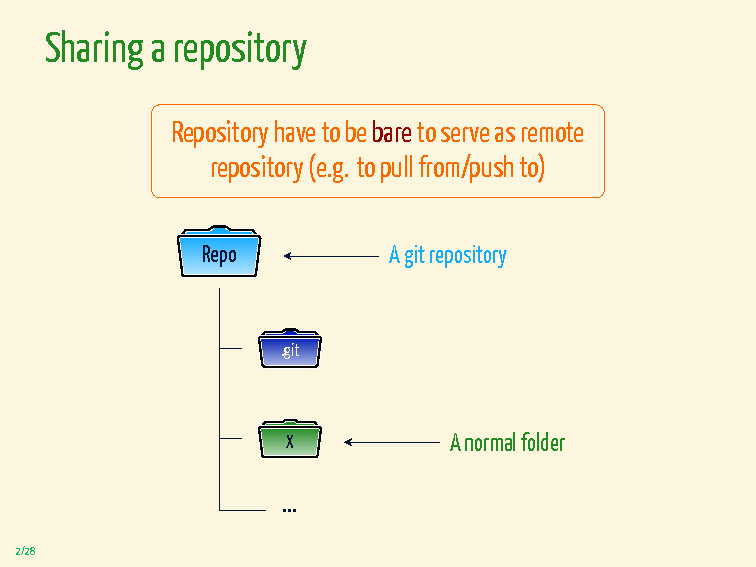
\includegraphics[width=0.8\textwidth, clip, trim=2cm 6mm 2cm 36mm]{Repository}};
            \begin{DrawOnNode}{fig}
                \fill[BGLIGHT] (0.3,0.9) rectangle (0.8,0.75);
                \draw[from] (0.33,0.84) -- node[pos=1, right, text=PS] {Workspace} ++(0.285,0);
                \draw[from] (0.44,0.56) -- node[pos=1, right, text=Navy, font=\small] {Local repository} ++(0.175,0);
                \draw[visible on=<2>, alert, thick] (0.26,0.48) rectangle (0.9,0.65) node[pos=0.5, above=0.06, font=\small]{Similar content as a bare repository};
                \fill[BGLIGHT, opacity=0.8, visible on=<2>]  (0,0) -- (1,0) -- (1,0.45) -- (0.22,0.45) -- (0.22,0.78) -- (1.0,0.78) -- (1,1) -- (0,1) -- cycle;
            \end{DrawOnNode}
        \end{tikzpicture}
    \end{center}
\end{frame}
%~~~~~~~~~~~~~~~~~~~~~~~~~~~~~~~~~~~~~~~~~~~~%
\begin{frame}[fragile]{How to create and use bare repositories?}
    \setlength{\leftmarginii}{8mm}
    \begin{overlayarea}{\textwidth}{0.8\textheight}
        \begin{onlyenv}<1>
            \vspace{1mm}
            \begin{itemize}
                \item By default it is not possible to push to a non-bare repository
                \item If you create a new repository in the browser on a platform like e.g. GitHub, you will not notice it, but a bare one will be created
                \item \alert{Bare repositories are meant} to serve as remote\\ \then i.e. \alert{to pull from and push to}
            \end{itemize}
            \vspace{1mm}
            \begin{enumerate}
                \item Initialize a bare empty repository, clone it, work and push to it
            \end{enumerate}
            \begin{lstlisting}[style=MyBash]
                $ mkdir <bare-repository>.git # .git is often used as suffix
                $ git init --bare <bare-repository>.git
                |+Initialised empty Git repository <bare-repository>.git+|
                $ git clone <bare-repository>.git <non-bare-repo>
                |+Cloning into '<non-bare-repo>'...
                warning: You appear to have cloned an empty repository.
                done.+|
                $ cd <non-bare-repo>
                # Work as usual and push when needed.
            \end{lstlisting}
        \end{onlyenv}
        \begin{onlyenv}<2->
            \begin{enumerate}
                \setcounter{enumi}{1}
                \item Initialize a bare empty repository and push an existing one to it
            \end{enumerate}
            \begin{lstlisting}[style=MyBash]
                $ mkdir <bare-repository>.git
                $ git init --bare <bare-repository>.git
                |+Initialised empty Git repository <bare-repository>.git+|
                $ cd <existent-non-bare-repository>
                $ git remote add origin /path/to/<bare-repository>.git
                $ git push -u origin main # <- From local desired branch
            \end{lstlisting}
            \vspace{1mm}
            \begin{uncoverenv}<3->
                \begin{enumerate}
                    \setcounter{enumi}{2}
                    \item Create a bare version of an existing non-bare one
                \end{enumerate}
                \begin{lstlisting}[style=MyBash]
                    $ git clone --bare <non-bare-repository> <bare-repository>.git
                    |+Cloning into bare repository 'QCD.git'...
                    done.+|
                    $ cd <non-bare-repository>
                    $ git remote add origin /path/to/<bare-repository>.git
                \end{lstlisting}
            \end{uncoverenv}
            \vspace{-1mm}
            \begin{varblock}{}[0.55\textwidth]{Pick your favourite way}<uncover@4>
                \small Probably options 2 and 3 are handier.
            \end{varblock}
        \end{onlyenv}
    \end{overlayarea}
    \FrameRemark{You can put your bare repository e.g.\ on a server or an external HDD (to clone on different machine without network).}
\end{frame}
%===============================================================%


%===============================================================%
\section{The remaining git commands}
%~~~~~~~~~~~~~~~~~~~~~~~~~~~~~~~~~~~~~~~~~~~~%
\begin{frame}[fragile]{You can now explore the rest alone!}
    \begin{tabular}{>{\bfseries\color{PB}}r>{\small}l}
        git mv       & Move or rename a file, a directory, or a symlink\\
        git restore  & Restore working tree files \Remark{we mentioned it already}\\
        git rm       & Remove files from the working tree and from the index\\
        git bisect   & Use binary search to find the commit that introduced a bug\\
        git grep     & Print lines matching a pattern\\
        \textcolor<2>{PT}{git rebase}   & Reapply commits on top of another base tip\\
        git reset    & Reset current HEAD to the specified state\\
        \textcolor<2>{PT}{git tag}      & Create, list, delete or verify a tag object signed with GPG\\
        git [...]    & Few more technical commands
    \end{tabular}
    \begin{varblock}{alert}[0.98\textwidth]{Wait for it!}<uncover@2>
        In the next and last part of the course we'll learn to rebase and tag
    \end{varblock}
\end{frame}
%===============================================================%


%===============================================================%
\section{Conclusions}
%~~~~~~~~~~~~~~~~~~~~~~~~~~~~~~~~~~~~~~~~~~~~%
\againframe<2>[plain]{Wow}
%~~~~~~~~~~~~~~~~~~~~~~~~~~~~~~~~~~~~~~~~~~~~%
\begin{frame}{That's \textbf{ALMOST} all folks}
    \vspace{-3mm}
    \begin{enumerate}[<+->]
        \item Start using Git.
              \alert{\textbf{Now.}}
              Not tomorrow or next week, today!\\
              $\to\;$ Repeat what done on these slides
        \item Was anything unclear?
              Did you get stuck at some point?\\
              $\to\;$ Drop me \PP{\href{mailto:sciarra@itp.uni-frankfurt.de}{{\small\faEnvelope}\;an email}}
        \item You can use Git to work in a very professional way!\\
              $\to\;$ Attend next part: \alert{\guillemotleft Git in real life\guillemotright}\tikzmark{tg}
    \end{enumerate}
    \begin{tikzpicture}[remember picture, overlay, scope on=<.->]
        \node[anchor=west, space=PT, text width=28mm] (content) at ($(tg)-(0.2,1.7)$) {
            git rebase\\
            git tag\\
            Semantic versioning\\
            Gitflow\\
        };
        \path[to, shorter={0mm}{1mm}] ($(tg)+(0.3,0.0)$) edge[out=0, in=90] (content.north);
    \end{tikzpicture}
    \par\vspace{-0.02\textheight}
    \begin{uncoverenv}<+->
        \begin{tikzpicture}[remember picture, overlay]
            \node[anchor=north east, cloud, aspect=3, cloud puffs=15, draw=PB, fill=PP!20, text=PB]
                at ($(current page.north east)+(-14mm,-6mm)$) {Thank you!};
            \node[left = of content, font=\large\bfseries, text=PQ] {Believe me, it's worth it!};
        \end{tikzpicture}
    \end{uncoverenv}
\end{frame}
%~~~~~~~~~~~~~~~~~~~~~~~~~~~~~~~~~~~~~~~~~~~~%

%===============================================================%

\end{document}
